\documentclass[11pt,a4paper]{article}

% ─── Encodage et langue ───
\usepackage[utf8]{inputenc}
\usepackage[T1]{fontenc}
\usepackage[french]{babel}

% ─── Maths ───
\usepackage{amsmath,amssymb}

% ─── Figures ───
\usepackage{graphicx}
\usepackage{subcaption}
\usepackage{float}
\graphicspath{{../figures/}{../experiments/01_instabilite/figures/}}

% ─── Schémas TikZ ───
\usepackage{tikz}
\usetikzlibrary{arrows.meta,positioning,fit,backgrounds,calc,decorations.pathreplacing}

% ─── Couleurs sémantiques ───
\definecolor{func}{HTML}{2166AC}
\definecolor{vect}{HTML}{B2182B}
\definecolor{mix}{HTML}{4DAF4A}
\definecolor{gris}{HTML}{666666}

% ─── Mise en page ───
\usepackage[margin=2.5cm]{geometry}
\usepackage{enumitem}
\usepackage{booktabs}
\usepackage{xcolor}
\usepackage{hyperref}
\hypersetup{colorlinks=true, linkcolor=blue!60!black, urlcolor=blue!70!black, citecolor=blue!60!black}
\usepackage{fancyhdr}
\usepackage{framed}

% ─── En-tête ───
\pagestyle{fancy}
\fancyhf{}
\fancyhead[L]{\small\textsc{Rapport de projet long}}
\fancyhead[R]{\small\textsc{Mars 2026}}
\fancyfoot[C]{\thepage}

% ─── Commandes ───
\newcommand{\Dw}{D_w}
\newcommand{\DK}{D_K}
\newcommand{\Dp}{D_p}
\newcommand{\Ltwo}{L^2(\mathcal{T})}

% Boîte fil rouge (règles scientifiques / rédactionnelles)
\newenvironment{filrouge}{%
  \def\FrameCommand{\fboxsep=8pt \fcolorbox{black!50}{yellow!10}}%
  \MakeFramed{\advance\hsize-\width \FrameRestore}%
  \noindent\ignorespaces
}{\endMakeFramed}

\title{%
  \vspace{-0.5cm}
  \textbf{Rapport de projet long}\\[0.3em]
  \small\textit{(Master TRIED)}\\[0.4em]
  \large ACP hybride et méthode des noyaux pour données mixtes\\
  fonctionnelles et vectorielles
}
\author{Pierre Chambet}
\date{Mars 2026}

\begin{document}
\maketitle
\thispagestyle{fancy}

\begin{abstract}
\noindent
\textbf{Contexte.}
Ce mémoire conclut le \textbf{projet long} du \textbf{Master TRIED}. Il s'intéresse
au \textbf{regroupement} de données (classification non supervisée) lorsque chaque
individu combine une partie \textbf{fonctionnelle} (une courbe) et une partie
\textbf{vectorielle} (un vecteur de covariables). La question est de savoir comment
utiliser \textbf{ensemble} ces deux types d'information pour former des groupes
cohérents, plutôt que de les traiter à part.

\end{abstract}

\vspace{0.75em}
\tableofcontents
\newpage

% ---------------------------------------------------------------------------
\section{Chapitre 1 : Introduction et formulation du problème}
% ---------------------------------------------------------------------------

\subsection{Contexte océanographique et acoustique}
En océanographie, une grandeur utile pour l'acoustique sous-marine est la
\emph{célérité} du son dans l'eau, obtenue à partir des champs physiques (par
exemple température, salinité) via une équation d'état. On peut alors s'intéresser
à des \emph{profils verticaux} de célérité, tout en disposant en parallèle
d'informations vectorielles (localisation, indices résumés, etc.). Les données
à traiter sont donc à la fois \textbf{fonctionnelles} (la courbe) et
\textbf{vectorielles} (le bloc de variables). L'enjeu du projet long est
d'étudier comment \textbf{regrouper} de tels individus \textbf{mixtes} avec des
méthodes adaptées, plutôt que de séparer artificiellement les deux types
d'information.

\subsection{Formulation statistique~: individu mixte \texorpdfstring{$(X,Z)$}{X,Z}}
On modélise chaque individu par un couple
\[
  (X,Z),\qquad X\in \mathbb{H}=\Ltwo,\qquad Z\in\mathbb{R}^p,
\]
où $X$ est une fonction observée sur un domaine $\mathcal{T}\subset\mathbb{R}$
(muni de la mesure usuelle pour définir l'espace de Hilbert $\mathbb{H}$), et
$Z$ est un vecteur de covariables dans $\mathbb{R}^p$. Un exemple possible
dans le cadre océanographique est un profil de célérité pour $X$ et des
variables résumées pour $Z$~; le reste du mémoire reste volontairement
\emph{général} pour s'attacher au problème statistique (coupler fonctionnel et
vecteur), indépendamment du détail d'une application.

\subsection{Deux mondes, une distance à construire}
Du point de vue mathématique, la difficulté centrale est que la structure
d'$\mathbb{H}$ (produit scalaire, distance $L^2$, possibilité de dériver pour
capturer la stratification) et la structure euclidienne de $\mathbb{R}^p$ ne
sont pas directement comparables. On ne dispose pas d'un espace produit canonique
où une norme unique agrégerait sans arbitrage l'écart fonctionnel et l'écart
vectoriel~: toute métrique sur le couple $(X,Z)$ est une \emph{construction},
paramétrée par des choix de poids, de normalisation, de filtrage par rapport à
la dérivée, ou par passage par des représentations intermédiaires (scores,
noyaux). La question «~comment faire coexister le continu et le discret~?~» est
donc le cœur du projet long~: il s'agit de définir des mesures de similarité
qui respectent à la fois la régularité fonctionnelle et la géométrie vectorielle,
sans fusion naïve qui laisserait l'une des modalités dominer l'autre par la
seule taille des composantes ou l'échelle de discrétisation.

\subsection{Évolution du stage et périmètre empirique}
Le projet long imposait l'exploration des données mixtes via une application au \textbf{SHOM} (Service hydrographique et océanographique de la Marine). Cependant, l'évaluation d'algorithmes non supervisés impliquant une vérité terrain absente de ces données brutes, l'étude s'est orientée vers des \textbf{jeux publics étiquetés} (jeux réels) et des données de \textbf{simulation} contrôlées. Le partitionnement reste néanmoins aveugle aux étiquettes, l'ARI n'intervenant qu'en stricte évaluation \emph{a posteriori}.

% ---------------------------------------------------------------------------
\section{Chapitre 2 : Architectures de distances et hybridation de surface}
% ---------------------------------------------------------------------------

\subsection{Lien avec la proposition de stage et chaîne de calcul}
Les constructions ci-dessous répondent au programme du projet long~: combiner
une composante fonctionnelle (profils lissés $X_i$) et un vecteur
$Z_i\in\mathbb{R}^p$. En pratique, les courbes sont d'abord lissées (splines,
représentation fonctionnelle discrète sur grille fine), puis une analyse en
composantes principales fonctionnelles (FPCA) fournit des scores pour la
stratégie~A et des évaluations $X_i(t)$, $X_i'(t)$ pour les
intégrales définissant $D_0$ et $D_1$. Cette réduction fonctionnelle est le
passage obligé annoncé dans le sujet lorsque l'on suit la voie «~discrétisation
puis méthodes euclidiennes~».

\subsection{Briques de niveau $0$~: $D_0$, $D_1$, $D_s$}
Nous partons de trois mesures complémentaires de dissimilarité~: écart global de niveau ($D_0$), écart de dynamique de forme ($D_1$), écart dans l'espace des covariables ($D_s$). Aucune ne suffit seule à résumer le couple $(X,Z)$~; la suite du chapitre ne fait qu'assembler ces briques selon des règles de fusion différentes.

On note $\mathcal{T}$ le domaine de la profondeur (ou du temps) et
$X_i,X_j\in \Ltwo$ les profils lissés.

\paragraph{Distance de niveau $D_0$.}
La distance $L^2$ entre courbes mesure l'écart global des profils~:
\begin{equation}
  D_0(i,j) = \sqrt{\int_{\mathcal{T}}
    \bigl[X_i(t)-X_j(t)\bigr]^2\,\mathrm{d}t } \, .
\end{equation}
Elle est sensible au décalage vertical entre trajectoires et moins à la seule
différence de forme lorsque les niveaux restent proches.

\paragraph{Distance de forme $D_1$.}
La dérivée première $X_i'$ encode la dynamique de stratification (taux de
variation du profil). On pose
\begin{equation}
  D_1(i,j) = \sqrt{\int_{\mathcal{T}}
    \bigl[X_i'(t)-X_j'(t)\bigr]^2\,\mathrm{d}t } \, .
\end{equation}
$D_1$ privilégie la proximité des formes au sens des gradients, au prix d'une
sensibilité accrue au bruit d'estimation si le lissage est insuffisant.

\paragraph{Distance vectorielle $D_s$.}
Les covariables $Z_i$ sont standardisées variable par variable (moyenne nulle,
variance unitaire), notées $Z_i^{\mathrm{std}}$. La distance euclidienne
associée est
\begin{equation}
  D_s(i,j) = \bigl\| Z_i^{\mathrm{std}} - Z_j^{\mathrm{std}} \bigr\|_2 \, .
\end{equation}
Elle ne dépend pas des courbes~; inversement, $D_0$ et $D_1$ ignorent $Z$.
Les trois briques sont donc \emph{complémentaires} mais prises isolément
\emph{non suffisantes} pour représenter la similarité du couple $(X,Z)$.

\subsection{Compromis fonctionnel $\Dp(\alpha)$ (niveau $1$)}
Les ordres de grandeur de $D_0$ et $D_1$ diffèrent en général~: sans mise à l'échelle,
un seul des deux termes pourrait dominer le mélange et fausser le sens du curseur
$\alpha$. On normalise donc par les maxima empiriques sur l'échantillon~:
\begin{equation}
  \tilde{D}_0 = \frac{D_0}{\max D_0}\,,\qquad
  \tilde{D}_1 = \frac{D_1}{\max D_1}\,,
\end{equation}
de sorte que $\tilde{D}_0$ et $\tilde{D}_1$ sont comparables (typiquement dans
$[0,1]$ hors diagonale). On combine ensuite les deux termes normalisés avec un
paramètre $\alpha\in[0,1]$ qui joue le rôle de \emph{curseur} entre niveau et forme~:
\begin{equation}
  \label{eq:Dp}
  \Dp(\alpha) = \sqrt{(1-\alpha)\,\tilde{D}_0^{\,2} + \alpha\,\tilde{D}_1^{\,2}}\,,
  \qquad \alpha\in[0,1] \, .
\end{equation}
Pour $\alpha=0$ (resp.\ $\alpha=1$), on retrouve $\tilde{D}_0$ (resp.\
$\tilde{D}_1$) à une normalisation près. Le paramètre $\alpha$ règle
exclusivement le compromis \emph{intra-fonctionnel} entre amplitude et
dynamique~; il ne mélange pas encore le fonctionnel avec le vectoriel.

\subsection{Pondération fonctionnel\,/\,vectorielle~: $\Dw(\alpha,\omega)$
(niveau $2$)}
On normalise également la partie vectorielle par le maximum empirique,
$\tilde{D}_s = D_s / \max D_s$, pour aligner l'échelle de $D_s$ sur celle des
distances fonctionnelles déjà calibrées. La distance mixte pondérée utilisée
dans la stratégie~B est
\begin{equation}
  \label{eq:Dw}
  \Dw(\alpha,\omega)
  = \sqrt{\omega\,\Dp(\alpha)^2 + (1-\omega)\,\tilde{D}_s^{\,2}}\,,
  \qquad \omega\in[0,1] \, .
\end{equation}
Ici $\alpha$ intervient dans $\Dp(\alpha)$ (choix niveau\,/\,forme dans le
bloc fonctionnel), tandis que $\omega$ pondère explicitement la contribution
de la partie fonctionnelle $\Dp(\alpha)$ par rapport à la partie vectorielle
$\tilde{D}_s$. Le symbole $\omega$ est réservé à cette distance $\Dw$~; au chapitre~3, le
coefficient $r$ du produit scalaire hybride~\eqref{eq:prodscalaire_hybride} joue
un tout autre rôle (pondération dans un produit scalaire théorique, pas dans
une matrice de distances PAM).

Sous les normalisations adoptées, $\Dw(\alpha,\omega)$ est une métrique sur les
deux composantes $\Dp(\alpha)$ et $\tilde{D}_s$~; elle peut donc alimenter un
partitionnement de type PAM (k-médoïdes) sur la matrice de dissimilarités complète.

\subsection{Noyaux produit et distance $\DK(\alpha)$}
On ne combine pas les distances comme dans~\eqref{eq:Dw}~: on suit la
construction de Ferreira \& de Carvalho (2014), imposée par le stage. On passe
par des \textbf{similarités} (plus grandes lorsque les individus sont proches)
dérivées de $\Dp(\alpha)$ et de $D_s$, on les multiplie, puis on en déduit une
matrice de distances pour le PAM.

On pose
\begin{align}
  K_f(i,j) &= \exp\!\left(-\frac{\Dp(\alpha)_{ij}^2}{2\sigma_f^2}\right)\,, \\
  K_s(i,j) &= \exp\!\left(-\frac{D_s(i,j)^2}{2\sigma_s^2}\right)\,,
\end{align}
avec $\sigma_f$ et $\sigma_s$ fixés par les médianes des distances non nulles sur
l'échantillon (deux échelles, une par bloc). Le score global est le produit
$K(i,j)=K_f(i,j)\,K_s(i,j)$. La matrice de distances associée est
\begin{equation}
  \label{eq:DK}
  \DK(i,j) = \sqrt{K(i,i)+K(j,j)-2K(i,j)}\,.
\end{equation}
Les noyaux gaussiens transforment chaque distance en similarité dans $[0,1]$~;
la médiane fixe un ordre de grandeur typique sans ajouter une grille de réglage
par jeu. Par rapport à la combinaison additive~\eqref{eq:Dw}, le produit $K_fK_s$
exige que les deux modalités soient \emph{simultanément} proches pour obtenir
une grande similarité globale.

\subsection{Stratégies A, B et C~: même ingrédients, géométries différentes}

\noindent
Les trois stratégies répondent au même besoin (fusionner $X$ et $Z$ pour le clustering) avec des géométries différentes~: A agrège des coordonnées dans un seul espace euclidien, B combine additivement des carrés de distances normalisées, C exige via le produit $K_f K_s$ que les deux modalités soient \emph{simultanément} proches. En pratique, nous ne les considérons pas comme interchangeables~: A est la ligne de référence ``réduction puis $k$-means''~; B offre un contrôle explicite de $\omega$ sur la dissimilarité PAM~; C, imposée par le cadre Ferreira \& de Carvalho (2014), est celle que les résultats agrégés du chapitre~5 tendent à favoriser lorsque le signal fonctionnel et vectoriel se combinent favorablement (sans écarter A lorsque le vecteur porte seul l'étiquette, voir S3 et Tecator).

\paragraph{Stratégie A (RS-PCA et $k$-means).}
La FPCA fournit $L$ scores $\xi_{i1},\ldots,\xi_{iL}$ par individu~; le vecteur
$Z_i$ est standardisé comme pour $D_s$. On forme le vecteur
$W_i = (\xi_{i1},\ldots,\xi_{iL},Z_{i1}^{\mathrm{std}},\ldots,Z_{ip}^{\mathrm{std}})$
dans $\mathbb{R}^{L+p}$, puis on centre-réduit chaque colonne de la matrice ainsi
construite. Le clustering est un $k$-means avec distance euclidienne, soit la
norme $\|\cdot\|_2$ sur l'espace des $W_i$. Il n'y a pas d'ACP séparée sur $Z$
dans cette chaîne de référence~: seule la FPCA résume le fonctionnel, le bloc
$Z$ restant en coordonnées physiques renormalisées. Du point de vue conceptuel,
c'est une fusion \emph{par concaténation} de coordonnées réduites, suivie d'une
norme euclidienne unique sur le vecteur agrégé.

\paragraph{Stratégie B (PAM sur $\Dw$).}
Pour chaque couple $(\alpha,\omega)$ d'une grille régulière ($21\times 21$
valeurs, pas $0{,}05$ sur $[0,1]$ pour chaque paramètre), on calcule la
matrice $\Dw(\alpha,\omega)$ et on applique PAM. La géométrie est entièrement
définie par la dissimilarité~\eqref{eq:Dw}, donc par une combinaison
\emph{additive} des carrés des contributions fonctionnelle et vectorielle après
normalisations.

\paragraph{Stratégie C (PAM sur $\DK$).}
La \textbf{stratégie~C} est le partitionnement PAM à partir de la matrice
$\DK(\alpha)$ construite comme en~\eqref{eq:DK} (noyaux produit de la
sous-section précédente). On balaie la même grille en $\alpha$ que pour $\Dp$
(21 valeurs, pas $0{,}05$)~; chaque valeur fixe $\Dp(\alpha)$, donc le noyau
$K_f$, avec $\sigma_f$ et $\sigma_s$ donnés par les médianes. La géométrie est
donc multiplicative ($K_fK_s$), par opposition à la combinaison additive de la
stratégie~B en~\eqref{eq:Dw}.

Aucune de ces trois procédures n'est intrinsèquement «~supérieure~» sur le plan
théorique~: elles traduisent des arbitrages géométriques distincts.

\subsection{Architecture à deux niveaux~: vue d'ensemble}

\begin{figure}[H]
\centering
\begin{tikzpicture}[
    base/.style={draw, rounded corners=4pt, minimum width=2.5cm, minimum height=0.9cm,
                 align=center, font=\small\bfseries},
    fleche/.style={-{Stealth[length=3mm]}, thick},
    etiq/.style={font=\footnotesize\itshape, text=gris},
  ]
  \node[base, fill=func!15, text=func]          (D0) at (0,0)     {$D_0$ \footnotesize niveau};
  \node[base, fill=func!15, text=func]          (D1) at (3.5,0)   {$D_1$ \footnotesize forme};
  \node[base, fill=vect!15, text=vect]          (Ds) at (8.5,0)   {$D_s$ \footnotesize vectoriel};
  \node[base, fill=func!25, text=func]          (Dp) at (1.75,-1.8) {$\Dp(\alpha)$};
  \node[base, fill=mix!20, text=mix!70!black]   (Dw) at (4.0,-3.6)  {$\Dw(\alpha,\omega)$};
  \node[base, fill=mix!20, text=mix!70!black]   (DK) at (7.5,-3.6)  {$\DK(\alpha)$};

  \draw[fleche, func!70] (D0) -- (Dp) node[etiq, midway, left=2pt]  {$1{-}\alpha$};
  \draw[fleche, func!70] (D1) -- (Dp) node[etiq, midway, right=2pt] {$\alpha$};
  \draw[fleche, func!70] (Dp) -- (Dw) node[etiq, midway, left=2pt]  {$\omega$};
  \draw[fleche, vect!70] (Ds) -- (Dw) node[etiq, midway, right=2pt] {$1{-}\omega$};
  \draw[fleche, func!70] (Dp) -- (DK) node[etiq, midway, left=2pt]  {$K_f$};
  \draw[fleche, vect!70] (Ds) -- (DK) node[etiq, midway, right=2pt] {$K_s$};

  \node[font=\footnotesize\scshape, text=gris] at (-1.5,0)    {Niv.~0};
  \node[font=\footnotesize\scshape, text=gris] at (-1.5,-1.8) {Niv.~1};
  \node[font=\footnotesize\scshape, text=gris] at (-1.5,-3.6) {Niv.~2};
\end{tikzpicture}
\caption{Architecture hiérarchique des distances~: cette figure résume le flux
$D_0,D_1,D_s \rightarrow \Dp \rightarrow \Dw$ ou $\DK$.
\textcolor{func}{Bleu}~= fonctionnel, \textcolor{vect}{rouge}~= vectoriel,
\textcolor{mix}{vert}~= mixte. Les niveaux 0 et 1 sont purement fonctionnels~;
le niveau~2 combine les deux sources.}
\label{fig:archi_distances}
\end{figure}

\begin{table}[H]
\centering
\begin{tabular}{lll}
  \toprule
  \textbf{Distance} & \textbf{Ce qu'elle voit} & \textbf{Ce qu'elle rate} \\
  \midrule
  $D_0$ & Niveau vertical des courbes & Forme / dynamique \\
  $D_1$ & Forme / vitesse de changement & Niveau vertical \\
  $D_s$ & Position dans $\mathbb{R}^p$ & Les courbes entièrement \\
  \bottomrule
\end{tabular}
\caption{Trois distances de base ($D_0$, $D_1$, $D_s$)~: elles se complètent et
aucune ne suffit seule pour résumer le couple $(X,Z)$.}
\label{tab:bilan_distances}
\end{table}

\begin{table}[H]
\centering
\renewcommand{\arraystretch}{1.25}
\begin{tabular}{l p{3.3cm} p{3.4cm} p{4.0cm}}
  \toprule
  \textbf{Stratégie} & \textbf{Représentation} &
  \textbf{Méthode de clustering} & \textbf{Fusion fonctionnel / vectoriel} \\
  \midrule
  A (FPCA$+Z$) &
  Vecteur $W = [\xi_{\text{FPCA}} \mid Z]$ standardisé &
  $k$-means (distance euclidienne) &
  Concaténation dans $\mathbb{R}^{L+p}$ \\
  B ($\Dw$) &
  Matrice de distances $\Dw(\alpha,\omega)$ &
  PAM (k-médoïdes) &
  Somme pondérée $\Dp(\alpha)^2 + \tilde{D}_s^2$ \\
  C ($\DK$) &
  Matrice de distances $\DK(\alpha)$ &
  PAM (k-médoïdes) &
  Produit de noyaux gaussiens $K_f \cdot K_s$ \\
  \bottomrule
\end{tabular}
\caption{Résumé des trois stratégies~: même ingrédients ($D_0$, $D_1$, $D_s$),
géométries de fusion différentes.}
\label{tab:strategies}
\end{table}

\subsection{Hybridation tardive et absence de covariance croisée}
Les stratégies A, B et C réalisent une hybridation \emph{tardive} : elles évaluent séparément les écarts fonctionnels et vectoriels avant de les fusionner. Par construction, aucune n'estime la covariance \emph{croisée} inter-blocs (tel le bloc $V_{yx}$ du chapitre suivant) avant de définir la métrique. Elles ignorent donc la structure potentielle de liaison statistique entre variations temporelles de $X$ et covariables $Z$. Cette limite fondamentale au niveau de la modélisation de surface motive l'ACP hybride (HFV) du chapitre~3, qui diagonalise explicitement une matrice de covariance jointe en amont du clustering.

% ---------------------------------------------------------------------------
\section{Chapitre 3 : ACP hybride fonctionnelle-vectorielle (HFV)}
% ---------------------------------------------------------------------------

\subsection{Pourquoi une autre géométrie que les distances du chapitre~2~?}
Les stratégies A, B et C construisent des dissimilarités à partir de résumés
déjà calculés séparément (FPCA d'un côté, $Z$ de l'autre), puis les combinent
ou les injectent dans des noyaux. L'ACP hybride (HFV) répond à une question
différente~: \emph{où} la variabilité commune entre les deux modalités est-elle
modélisée avant toute distance de clustering~? L'idée est d'estimer une
\emph{covariance jointe} sur des coordonnées réduites, puis de diagonaliser
cette matrice pour obtenir des axes qui mélangent explicitement les deux
blocs. La présentation qui suit enchaîne les étapes dans l'ordre du calcul.

\subsection{Intuition~: espace hybride $\mathbb{H}$}
En théorie, l'individu est une paire $(X,Z)$ dans un espace de Hilbert
$\mathbb{H}$ mélangeant une composante fonctionnelle ($L^2$) et une composante
vectorielle ($\mathbb{R}^p$). On introduit un produit scalaire hybride qui
additionne la partie continue et la partie discrète, avec un coefficient
positif calibrant le poids relatif du vectoriel~:
\begin{equation}
  \label{eq:prodscalaire_hybride}
  \langle h_1, h_2 \rangle_{\mathbb{H}}
  = \langle f_1, f_2 \rangle_{\mathbb{F}}
  + r\,\langle v_1, v_2 \rangle_{\mathbb{R}^p}\,,
\end{equation}
de sorte qu'aucune modalité n'écrase l'autre par la seule échelle de mesure.

\subsection{L'estimation matricielle en trois temps}
Le modèle en dimension infinie se ramène à un vecteur de dimension finie
$(L{+}J)$ par individu.

\paragraph{Étape 1 : réduction séparée.}
Une FPCA sur les courbes lissées fournit $L$ scores par individu,
$\eta_{i1},\ldots,\eta_{iL}$, sur les fonctions de base de la FPCA,
$\phi_1,\ldots,\phi_L$. Le vecteur $Z$ est centré et réduit, puis résumé par une
ACP classique en $J$ scores
$\gamma_{i1},\ldots,\gamma_{iJ}$.

\paragraph{Calibration du coefficient $r$.}
Les échelles de dispersion (variances) des résumés fonctionnels et vectoriels diffèrent considérablement. 
Afin d'éviter que l'une n'écrase algébriquement l'autre lors de la définition de la géométrie jointe, 
on introduit un simple ratio de pondération empirique $r$. Celui-ci correspond au strict rapport des variances 
des blocs respectifs \emph{avant} fusion :
\begin{equation}
  \label{eq:r_trace}
  r = \frac{\mathrm{tr}\,\mathrm{Cov}(\eta)}{\mathrm{tr}\,\mathrm{Cov}(\gamma)}\,.
\end{equation}
Ce ratio $r$ permet d'équilibrer et de fixer mathématiquement le poids relatif des deux produits scalaires.

\paragraph{Étape 2 : vecteur d'état joint.}
On encode ce poids en posant $\tilde{\gamma}_{ij} = \sqrt{r}\,\gamma_{ij}$~: la
norme euclidienne sur le vecteur concaténé reproduit alors le facteur $r$ du
produit scalaire hybride~\eqref{eq:prodscalaire_hybride}. On concatène les
deux blocs en un seul vecteur de $\mathbb{R}^{L+J}$~:
\begin{equation}
  x_i = (\eta_{i1},\ldots,\eta_{iL},\tilde{\gamma}_{i1},\ldots,\tilde{\gamma}_{iJ})\,.
\end{equation}

\paragraph{Étape 3 : covariance des coordonnées réduites.}
On centre les colonnes de la matrice des $x_i$, puis on estime la covariance
empirique en notant les $x_i$ comme vecteurs colonnes centrés~:
\begin{equation}
  V = \frac{1}{n-1}\sum_{i=1}^n x_i x_i^{\top}\,.
\end{equation}
Elle admet la partition par blocs fonctionnel / vectoriel~:
\begin{equation}
  \label{eq:Vblocs}
  V = \begin{bmatrix} V_y & V_{yx} \\ V_{xy} & V_x \end{bmatrix}\,,
\end{equation}
où $V_y$ et $V_x$ portent la variabilité propre à chaque modalité. Le bloc
croisé vérifie $V_{yx} = V_{xy}^{\top}$ et mesure la \emph{covariance croisée}
entre scores fonctionnels et scores vectoriels~: c'est le bloc qui manquait aux
constructions «~de surface~» du chapitre~2. Tant que $V_{yx}$ n'est pas nul, les
fluctuations des deux sources ne sont pas traitées comme indépendantes au moment
de définir la géométrie jointe.

\subsection{Axes principaux et structure des vecteurs propres}
Les directions de variance maximale sous contrainte de norme~1 sont les
vecteurs propres de $V$ (théorème spectral)~: pour un axe $m$, la variance
projetée s'écrit $\langle e_m, V e_m\rangle$. Chaque vecteur propre se décompose
selon les deux blocs~:
\begin{equation}
  e_m = \begin{bmatrix} c_m \\ d_m \end{bmatrix}\,,
  \qquad c_m\in\mathbb{R}^L\,,\quad d_m\in\mathbb{R}^J\,,
\end{equation}
ce qui signifie qu'un axe dominant peut combiner à la fois un motif sur les
scores FPCA et un motif sur les scores vectoriels ; ce n'est pas une suite
«~d'abord fonctionnel, puis vectoriel~», mais une \emph{intrication} dans un
repère orthogonal commun.

\subsection{Scores hybrides et reconstruction}
Le score de l'individu $i$ sur l'axe $m$ est la coordonnée sur $e_m$, soit la
projection de $x_i$ sur cet axe~:
\begin{equation}
  \rho_{im}
  = \sum_{h=1}^L \eta_{ih}\,c_{mh}
  + \sum_{j=1}^J \tilde{\gamma}_{ij}\,d_{mj}
  = \sum_{h=1}^L \eta_{ih}\,c_{mh}
  + \sqrt{r}\,\sum_{j=1}^J \gamma_{ij}\,d_{mj}\,.
\end{equation}
La partie fonctionnelle de l'axe se lit comme une fonction dans $\Ltwo$ en
combinant les fonctions de base de la FPCA~:
\begin{equation}
  \psi_m(t) = \sum_{h=1}^L c_{mh}\,\phi_h(t)\,.
\end{equation}
La partie vectorielle se lit dans $\mathbb{R}^p$ en combinant les directions
principales de l'ACP sur $Z$ (vecteurs propres unitaires de la covariance
empirique de $Z$ standardisé), notées $w_1,\ldots,w_J$~:
\begin{equation}
  \label{eq:theta_m}
  \theta_m = \sum_{j=1}^J d_{mj}\,w_j\,.
\end{equation}
Ainsi $\rho_{im}$ est bien la somme des contributions fonctionnelle (via les
$\eta_{ih}$ et $c_{mh}$) et vectorielle (via les $\tilde{\gamma}_{ij}$ et
$d_{mj}$), et la reconstruction «~lisible~» de l'axe $m$ sépare explicitement
$\psi_m$ (continu) et $\theta_m$ (discret dans $\mathbb{R}^p$), sans passer par
un retour mécanique aux $p$ coordonnées brutes de $Z$ si l'on reste dans le
sous-espace des $J$ premières composantes. Dans la mise en œuvre numérique du
stage, ce sont surtout les courbes qui sont reconstruites explicitement dans
$L^2$ à partir des loadings sur les $\phi_h$~; la composante vectorielle se
déduit des scores $\gamma_{ij}$ et des $d_{mj}$, ou du profil $\theta_m$, plutôt
qu'un vecteur $Z$ entier réaffiché dans $\mathbb{R}^p$ à chaque étape.

Les courbes reconstruites à partir des composantes hybrides restent dans le
sous-espace engendré par les $(\phi_h)$, mais les coefficients ne sont
plus ceux de la seule FPCA initiale~: ils sont \emph{informés} par la structure
de liaison entre $\eta$ et $\gamma$ contenue dans $V$, en
particulier dans $V_{yx}$.

\subsection{De la reconstruction HFV à la matrice de distances noyau}
\label{sec:hfv_noyaux_D1}
Une fois les trajectoires reconstruites dans le sous-espace engendré par les
$(\phi_h)$ à partir des scores hybrides, on mesure une dissimilarité de type
$L^2$ discrétisée entre les courbes reconstruites, notée
$\mathcal{D}_{\mathrm{recon}}$. Sur le bloc vectoriel $Z$ (standardisé), on
utilise la distance euclidienne usuelle $\mathcal{D}_Z$. À chaque bloc on
associe un noyau gaussien (écarts-types $\sigma_f$ et $\sigma_s$ fixés à partir
des médianes des distances intra-bloc), on forme le produit des noyaux comme
au chapitre~2 pour~\eqref{eq:DK}, puis une matrice de distances
$\mathcal{D}_K$ induite par ce noyau hybride. Le partitionnement est réalisé par
une méthode adaptée aux matrices de dissimilarités (PAM), avec le même nombre
de groupes $k$ que pour les autres stratégies comparées.

% ---------------------------------------------------------------------------
\section{Chapitre 4 : Dispositif empirique et verrou du non-supervisé}
% ---------------------------------------------------------------------------

\subsection{Les données d'étude (Le Matériel)}
\label{sec:materiel}

Pour \textbf{tester} le pipeline et \textbf{mesurer} les comportements des
méthodes (ARI, matrices de confusion, etc.), on s'appuie sur des \textbf{données
étiquetées} (réelles ou simulées) en réservant les labels à
l'évaluation, pas au choix des hyperparamètres. La seule voie pour \emph{fixer}
simultanément le nombre de groupes $K$, la séparation entre classes sur la
composante fonctionnelle et sur le vecteur $Z$, et les niveaux de bruit, est
l'expérimentation sur données simulées dont la loi est connue par construction.

La simulation retenue s'appuie sur un générateur de courbes simulées avec bruit contrôlé~: courbes discrétisées sur une grille de temps
$(t_1,\ldots,t_N)$ sur $[0,1]$ ($N=60$) dans une base trigonométrique,
coefficients de classe modulés par $\delta=(\delta_1,\delta_2,\delta_3)$, où
$\delta_1$ et $\delta_2$ règlent l'écart des coefficients fonctionnels (niveau
et dynamique de forme dans le générateur) et $\delta_3$ la séparation des
moyennes du bloc $Z$. Le bloc $Z\in\mathbb{R}^p$ ($p=20$) est bruité par un
gaussien additif de variance $\tau^2$~; le signal fonctionnel observé l'est
également par un \textbf{bruit gaussien} additif de variance $\sigma^2$. Les
effectifs par classe sont égaux ($100$ individus par classe, $n=300$) et le
nombre de groupes simulé est $K=3$. Quatre scénarios S1-S4 font varier les
$\delta$ (tableau~\ref{tab:materiel_experimental}).

Les \textbf{trois jeux réels} publics (Canadian Weather, Berkeley Growth,
Tecator) offrent des étiquettes de référence consensuelles pour une
\textbf{évaluation a posteriori par ARI} sans participer au réglage des
hyperparamètres. Le tableau~\ref{tab:materiel_experimental} récapitule à la fois
les scénarios simulés et les trois jeux réels.

\begin{table}[H]
\centering
\setlength{\tabcolsep}{7pt}
\renewcommand{\arraystretch}{1.15}
\begin{tabular*}{\textwidth}{@{\extracolsep{\fill}}lcccc@{}}
  \toprule
  \multicolumn{5}{@{}l}{\textbf{Bloc 1 : données simulées}} \\
  \midrule
  \textbf{Scénario} & $\delta_1$ & $\delta_2$ & $\delta_3$ & \textbf{Effectif / $K$} \\
  \midrule
  S1 & $1{,}0$ & $1{,}0$ & $1{,}0$ & $n=300$, $K=3$ \\
  S2 & $1{,}0$ & $1{,}0$ & $0{,}5$ & id. \\
  S3 & $0{,}5$ & $0{,}5$ & $1{,}0$ & id. \\
  S4 & $0{,}5$ & $0{,}5$ & $0{,}5$ & id. \\
  \midrule
  \multicolumn{5}{@{}l}{\textbf{Bloc 2 : jeux réels}} \\
  \midrule
  \textbf{Jeu} & \textbf{Courbes $X(t)$} & $n$ & \textbf{Covariables $Z$} & \textbf{$k$ / classes} \\
  \midrule
  Canadian Weather & Temp.\ annuelle & 35 & lat., long., précip. & 4 régions \\
  Berkeley Growth & Courbe taille-âge & 93 & taille fin., croiss. & 2 (sexe) \\
  Tecator & \shortstack[l]{Absorbance NIR\\selon longueur d'onde} & 215 & eau, protéines & 3 (gras) \\
  \bottomrule
\end{tabular*}
\caption{Matériel expérimental : scénarios simulés ($\delta_1$ niveau fonctionnel,
$\delta_2$ forme, $\delta_3$ séparation sur $Z$) et jeux réels utilisés aux
chapitres~5 et~6. Pour Tecator, la partie fonctionnelle est l'absorbance mesurée
en fonction de la longueur d'onde (un spectre par individu).}
\label{tab:materiel_experimental}
\end{table}

Pour chaque scénario simulé, le benchmark répète $50$ fois la chaîne complète
(lissage, FPCA, distances, stratégies A/B/C et chaîne HFV) avec des graines
indépendantes. Les hyperparamètres dépendant de la silhouette sont cherchés sur
la même grille discrète que le pipeline principal (pas $0{,}05$ sur $[0,1]$)~;
l'ARI sert \emph{uniquement} à l'évaluation.

\begin{figure}[H]
  \centering
  
\includegraphics[width=0.88\textwidth]{canadian_weather/fig02_courbes_regions.png}
  \caption{Canadian Weather : séparation visuelle des profils
  entre les quatre régions retenues comme vérité de groupe pour l'ARI (35 courbes de
  température annuelle lissées)~; elle illustre le jeu du tableau~\ref{tab:materiel_experimental}.}
  \label{fig:canadian_descriptif}
\end{figure}

\subsection{Le verrou du calibrage}
Les hyperparamètres $k$, $\alpha$ et $\omega$ conditionnent l'intégralité de la partition induite. En l'absence de labels opérationnels, l'optimisation des stratégies A, B et C s'appuie obligatoirement sur des critères internes (ex: silhouette ou instabilité bootstrap). La chaîne HFV, quant à elle, calibre son ratio interne $r$ en amont sans nécessiter de recherche sur $(\alpha, \omega)$. Dans tout le pipeline de ce dispositif, l'ARI reste strictement confiné à un rôle d'évaluation extérieure et ne participe jamais à la calibration.

\subsection{Le paradoxe de la silhouette}
\label{sec:silhouette}
Étant donnée une matrice de distances $D$ et une partition
$\mathcal{C}=\{C_1,\ldots,C_k\}$, la silhouette de l'individu $i$ affecté au
cluster $C_\ell$ compare la cohésion intra-groupe à la séparation inter-groupes~:
\begin{equation}
  s(i) = \frac{b(i)-a(i)}{\max\{a(i),\,b(i)\}}\,,
\end{equation}
où $a(i)$ est la distance moyenne de $i$ aux autres points de $C_\ell$ et $b(i)$
la distance moyenne minimale aux points d'un autre cluster. La silhouette moyenne $\bar{s}=\frac{1}{n}\sum_i s(i)$ synthétise la
qualité géométrique de la partition \emph{dans la métrique choisie}. Le protocole
classique du projet maximise $\bar{s}$ sur une grille de $(\alpha,\omega)$ à
$k$ fixé, ce qui est cohérent avec une recherche de groupes compacts et bien
séparés \emph{au sens de $D$}.

% ---------------------------------------------------------------------------
% Fichier généré — NE PAS ÉDITER À LA MAIN
% Généré le : 2026-03-22 15:14:51 CET
% Git : 394a048
% Regénérer : Rscript scripts/generate_rapport_stage_paradox_tex.R
% ---------------------------------------------------------------------------

\begin{table}[H]
  \centering
  \small
  \renewcommand{\arraystretch}{1.2}
  \begin{tabular}{llccccccc}
    \toprule
    \textbf{Jeu} & $K$
    & \multicolumn{3}{c}{\textbf{Choix par silhouette} ($\Dw$, PAM)}
    & \multicolumn{3}{c}{\textbf{Maximum d'ARI sur la grille} (éval.)}
    & $\Delta$\,ARI \\
    \cmidrule(lr){3-5}\cmidrule(lr){6-8}
    & & $(\alpha,\omega)$ & $\bar s$ & ARI & $(\alpha,\omega)$ & $\bar s$ & ARI & \\
    \midrule
  Canadian Weather & 4 & $(0{,}00,0{,}00)$ & 0{,}448 & 0{,}616 & $(0{,}55,0{,}80)$ & 0{,}311 & 0{,}898 & 0{,}283 \\
  AEMET & 4 & $(0{,}00,1{,}00)$ & 0{,}464 & 0{,}167 & $(0{,}85,0{,}15)$ & 0{,}359 & 0{,}434 & 0{,}266 \\
  Growth & 2 & $(0{,}00,0{,}00)$ & 0{,}554 & 0{,}424 & $(0{,}85,0{,}30)$ & 0{,}372 & 0{,}756 & 0{,}332 \\
  Tecator & 3 & $(0{,}00,1{,}00)$ & 0{,}509 & 0{,}151 & $(1{,}00,1{,}00)$ & 0{,}248 & 0{,}626 & 0{,}475 \\
    \bottomrule
  \end{tabular}
  \caption{Paradoxe silhouette\,/\,ARI sur la stratégie~B ($\Dw$, grille $21\times 21$, pas $0{,}05$, $k=K$ fixé à la vérité terrain pour l'évaluation).
  Le bloc central droit (maximum d'ARI sur la grille) est un \emph{contrefactuel}~:
  il suppose que l'on pourrait optimiser $(\alpha,\omega)$ pour l'ARI, ce qui exige des étiquettes et ne correspond pas au réglage non supervisé.
  La dernière colonne donne $\Delta\mathrm{ARI} = \mathrm{ARI}_{\max} - \mathrm{ARI}_{\mathrm{sil}}$ (toujours $\ge 0$).}
  \label{tab:paradox_silhouette_ari}
\end{table}



Le point critique est que la silhouette $\bar{s}$ juge exclusivement la \emph{séparation géométrique} conférée par la métrique employée. Une distance favorisant des amas compacts et sphériques obtiendra souvent une excellente silhouette, même si elle fragmente artificiellement les véritables sous-classes allongées. Ainsi, le couple $(\alpha,\omega)$ maximisant $\bar{s}$ tend régulièrement à écraser l'une des dimensions (privilégiant par exemple le seul bloc discret) au détriment de l'information de forme requise pour maximiser l'ARI.

\medskip
\noindent
À $k$ fixé, le tableau~\ref{tab:paradox_silhouette_ari} illustre ce phénomène sur la stratégie~B~: le choix opérationnel par silhouette s'écarte systématiquement de l'optimum \emph{contrefactuel} par ARI. L'écart $\Delta\mathrm{ARI}$ quantifie empiriquement ce coût. Ce constat impose de calibrer en priorité le paramètre macroscopique le plus structurant~: le nombre de groupes $k$.

\subsection{Stabilisation par instabilité bootstrap (Fang \& Wang)}
\label{sec:fang_wang}

Puisque la silhouette s'avère fragile pour calibrer conjointement les poids géométriques, l'approche retenue est celle, complémentaire et non-supervisée, de \textbf{Fang \& Wang}~: minimiser l'\emph{instabilité} des partitions évaluée par ré-échantillonnage bootstrap. Un $k$ induisant des affectations très variables d'un tirage à l'autre est rejeté au profit du $k$ le plus robuste, sans recours aux étiquettes. Ce critère reste toutefois une heuristique dont le comportement se dégrade lorsque le signal de groupe s'effondre (S3-S4, chapitre~5).

\paragraph{Procédure de Fang \& Wang.}
Fang et Wang proposent de sélectionner $k$ en \emph{minimisant} une instabilité
de clustering estimée par bootstrap. L'idée s'oppose aux procédures qui
\emph{maximisent} une similarité avec une partition de référence inconnue~: deux
échantillons bootstrap indépendants de taille $n$ sont tirés avec remise~; on
clusterise chacun avec le même algorithme et le même $k$ sur la matrice de
distances restreinte aux individus tirés, puis on compare les deux partitions
après avoir prolongé les affectations à l'ensemble observé (classification des
points non tirés au médoïde ou au centre le plus proche dans l'espace des
distances). La désagrégation moyenne sur $B$ répétitions donne une estimation
$\mathrm{Inst}(k)$ de l'instabilité attendue pour ce $k$. Le nombre de
clusters retenu est
\begin{equation}
  k_{\mathrm{opt}} \in \arg\min_{k\in\mathcal{K}} \mathrm{Inst}(k)\,,
\end{equation}
où $\mathcal{K}$ est un ensemble fini de candidats. Dans ce mémoire, on fixe $\mathcal{K}=\{2,\ldots,6\}$.

\paragraph{Mécanique du bootstrap.}
Formellement, pour un algorithme de clustering $\mathcal{A}$ et une distance
$D$ fixées, l'instabilité (au sens de Wang, estimée par bootstrap dans Fang \&
Wang) est liée à la variabilité des partitions induites par deux échantillons
indépendants de même loi empirique. Si l'on note $\mathcal{P}^{(1)}_b$ et
$\mathcal{P}^{(2)}_b$ les partitions obtenues à la répétition $b$ après extension
commune sur $\{1,\ldots,n\}$, et $\delta(\cdot,\cdot)$ une mesure de désaccord
entre partitions (basée sur les co-affectations de paires), l'estimateur
utilisé est de la forme
\begin{equation}
  \mathrm{Inst}(k)
  = \frac{1}{B}\sum_{b=1}^B \delta\!\left(\mathcal{P}^{(1)}_b,\mathcal{P}^{(2)}_b\right)\,.
\end{equation}
Un $k$ trop petit peut fusionner des modes réels et paraître stable~; un $k$ trop
grand fragmente le bruit et peut aussi instabiliser les frontières.

\paragraph{Couplage avec la grille \texorpdfstring{$(\alpha,\omega)$}{(alpha, omega)} et rôle de l'évaluation.}
\emph{Côté calcul}, la matrice $\Dw(\alpha,\omega)$ dépend du couple
$(\alpha,\omega)$~: pour chaque point de grille, on calcule $D$, puis
$\mathrm{Inst}(k)$ sur les candidats $k\in\mathcal{K}$ et l'on obtient
$k_{\mathrm{opt}}(\alpha,\omega)$. L'ordre opérationnel est donc une boucle sur
$(\alpha,\omega)$ avec comparaison des $k$ à l'intérieur, et non un $k$ unique
fixé une fois pour toutes avant toute grille. On obtient ainsi une carte
$(\alpha,\omega)\mapsto k_{\mathrm{opt}}$ et des représentations
d'instabilité (heatmaps) utiles au diagnostic. Les étiquettes, lorsqu'elles
existent, ne participent pas à ce choix~: elles servent uniquement à calculer
l'ARI ou des matrices de confusion \emph{après} fixation de
$(k,\alpha,\omega)$.

\paragraph{Illustration sur les jeux réels.}
Comme annoncé en section~\ref{sec:silhouette}, l'illustration sur la grille
$(\alpha,\omega)$ repose sur l'instabilité bootstrap, et non sur
une carte de silhouette. Les calculs numériques utilisent $B=150$ répétitions bootstrap, la grille
$(\alpha,\omega)$ de $21\times 21$ points sur $[0,1]$ (pas $0{,}05$) et des
candidats $k\in\{2,\ldots,6\}$, avec PAM sur $\Dw(\alpha,\omega)$ comme dans le
reste du pipeline. La figure~\ref{fig:instab_reels} juxtapose les trois jeux
réels du tableau~\ref{tab:materiel_experimental}~: chaque planche regroupe cinq cartes
$(\alpha,\omega)$, une par valeur de $k$ testée, plus une légende. L'échelle
de couleur encode l'instabilité estimée (bleu~: faible, rouge~: forte)~; le
symbole $\times$ indique le couple $(\alpha,\omega)$ qui minimise l'instabilité
\emph{pour le $k$ correspondant}. La juxtaposition met en évidence que la
forme des zones ``favorables'' varie fortement d'un jeu à l'autre (nombre de
classes de référence, géométrie du signal fonctionnel et du bloc $Z$), alors
que le protocole reste identique.

\begin{figure}[H]
  \centering
  \begin{subfigure}[t]{0.48\textwidth}
    \centering
    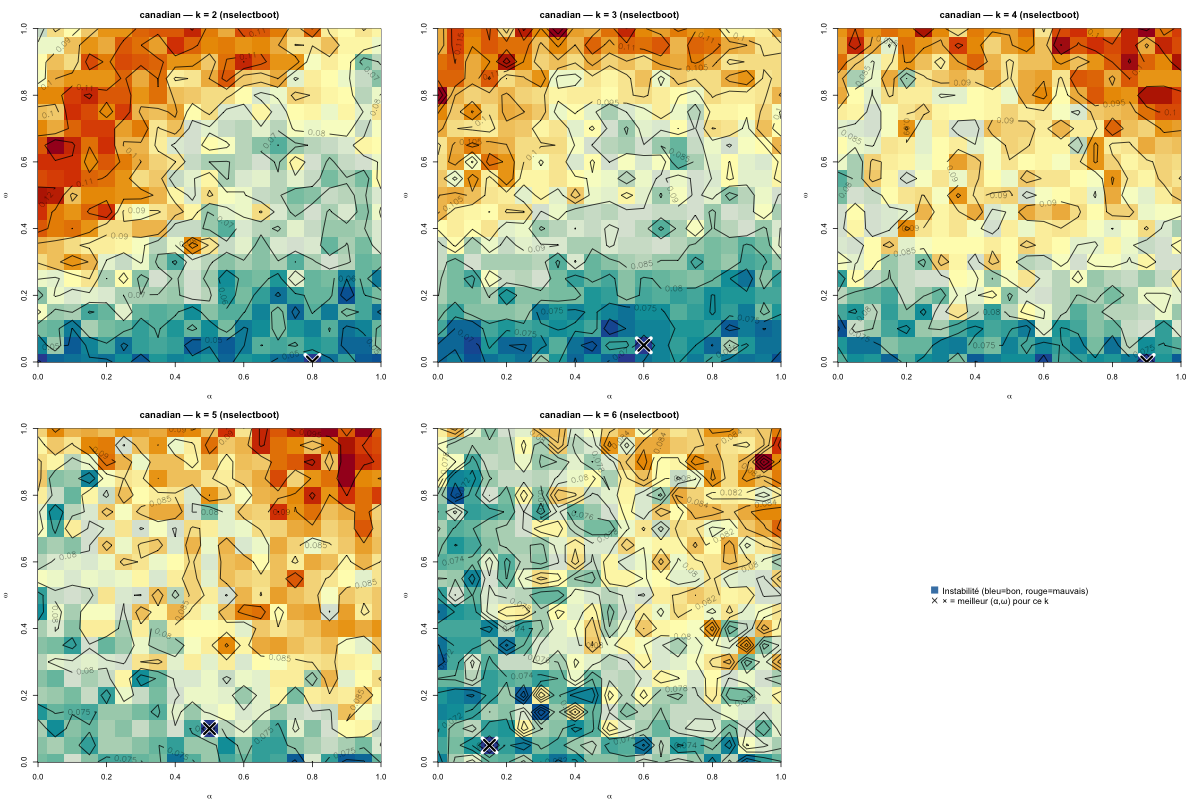
\includegraphics[width=\linewidth]{nselectboot_heatmap_canadian.png}
    \caption{Canadian Weather ($K=4$ régions).}
    \label{fig:instab_canadian}
  \end{subfigure}\hfill
  \begin{subfigure}[t]{0.48\textwidth}
    \centering
    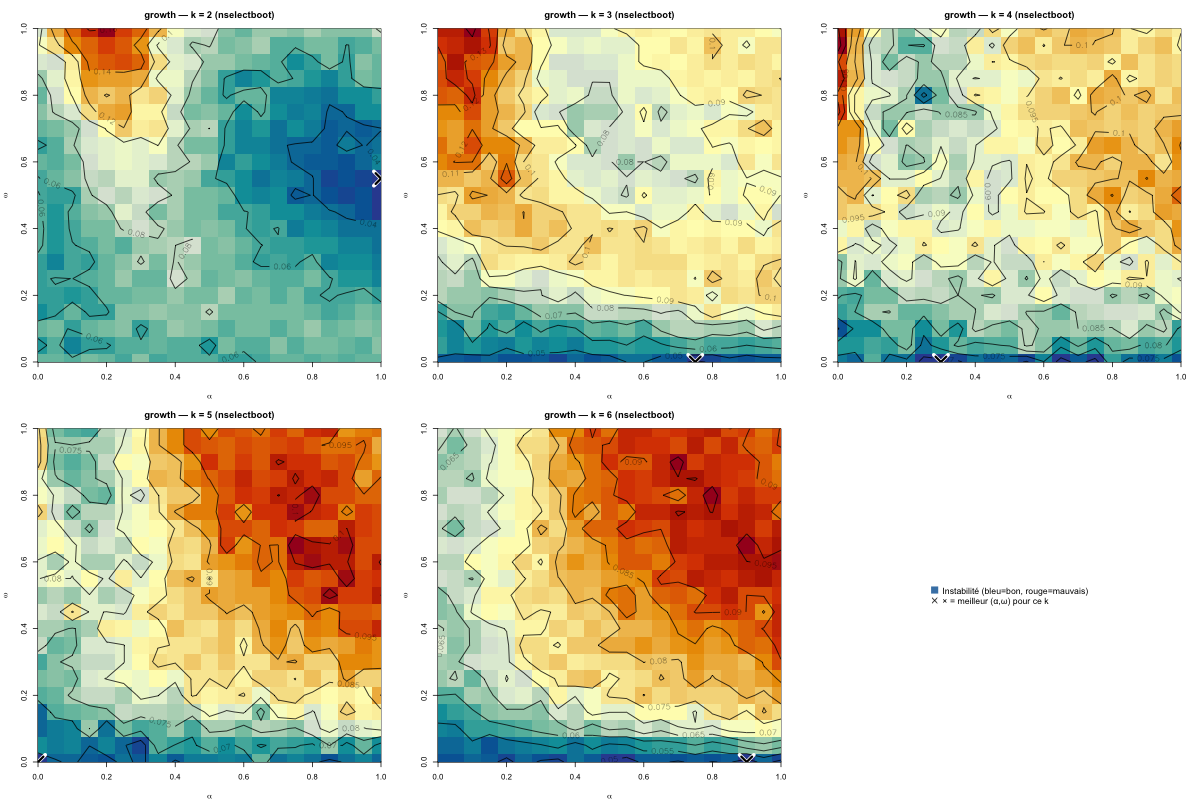
\includegraphics[width=\linewidth]{nselectboot_heatmap_growth.png}
    \caption{Growth ($K=2$, sexe).}
    \label{fig:instab_growth}
  \end{subfigure}

  \vspace{0.75em}

  \null\hfill
  \begin{subfigure}[t]{0.48\textwidth}
    \centering
    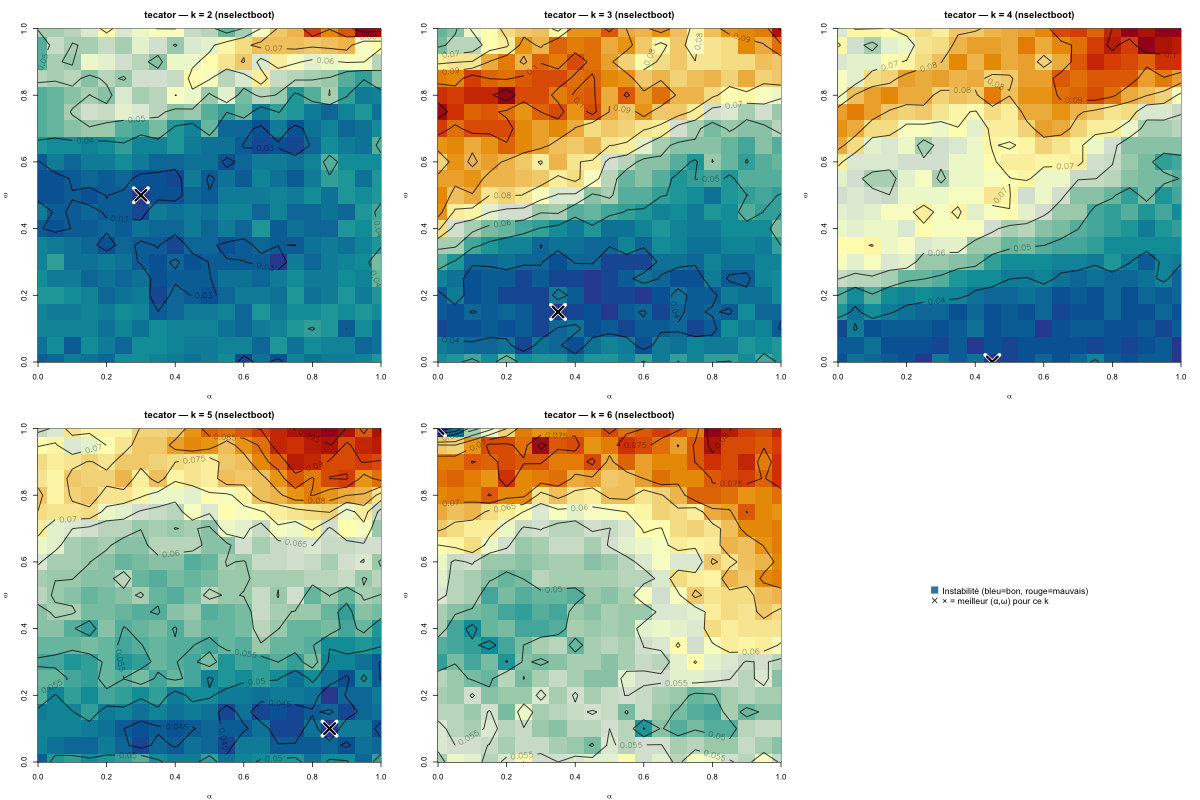
\includegraphics[width=\linewidth]{nselectboot_heatmap_tecator.png}
    \caption{Tecator ($K=3$ classes de teneur en matières grasses).}
    \label{fig:instab_tecator}
  \end{subfigure}
  \hfill\null
  \caption{Instabilité bootstrap (Fang \& Wang) sur $\Dw$ pour les trois jeux
  réels~: cette figure montre comment les zones de faible instabilité (bleu) et forte instabilité (rouge)
  se réorganisent selon le jeu et selon $k$~; le symbole $\times$ marque le couple $(\alpha,\omega)$
  qui minimise l'instabilité pour le $k$ de la planche. Comparaison directe des cartes par $k$ et par $(\alpha,\omega)$.}
  \label{fig:instab_reels}
\end{figure}

Le même protocole d'instabilité bootstrap (grille $(\alpha,\omega)$, PAM sur
$\Dw$, candidats $k\in\{2,\ldots,6\}$, $B=150$) est appliqué aux quatre
scénarios S1-S4 issus des données simulées décrits section~\ref{sec:materiel}. Les
heatmaps par scénario et l'interprétation quantitative (alignement de
$k_{\mathrm{opt}}$ avec le vrai $K=3$) sont présentées en
section~\ref{sec:instab_simule} du chapitre~5 (figure~\ref{fig:instab_simule}).

\medskip
\noindent
En synthèse : (i)~la silhouette reste un critère interne lisible mais sujette au
paradoxe de la séparation géométrique~; (ii)~le choix de $k$ à $(\alpha,\omega)$
fixé peut s'appuyer sur la minimisation de l'instabilité au sens de Fang \&
Wang~; (iii)~l'ARI et les partitions de référence restent des outils
d'\emph{évaluation}, pas d'optimisation opérationnelle en contexte non
étiqueté. Les chapitres~5 et~6 rapportent les performances sur ce matériel.

% ---------------------------------------------------------------------------
\section{Chapitre 5 : Données simulées}
\label{sec:chap5_donnees_simulees}
% ---------------------------------------------------------------------------

\subsection{Instabilité bootstrap sur les scénarios simulés}
\label{sec:instab_simule}

Les mêmes principes qu'en section~\ref{sec:fang_wang} (grille en $(\alpha,\omega)$,
PAM sur $\Dw$, recherche de $k$ par instabilité bootstrap) ont été appliqués aux
données simulées, en quatre scénarios S1-S4. Un bilan agrégé (une graine par scénario)
indique~: pour S1, environ $91\,\%$ des couples $(\alpha,\omega)$ sélectionnent le
$k_{\mathrm{opt}}$ égal au vrai $k=3$~; pour S2, environ $72\,\%$~; pour S3, la
proportion tombe à environ $8\,\%$ et la médiane de $k_{\mathrm{opt}}$ se
décale vers des valeurs trop grandes~; pour S4, aucun couple ne retient
$k=3$ (médiane et mode vers $6$). La figure~\ref{fig:instab_simule} montre, pour
chaque scénario, les cartes d'instabilité par $k$ sur la grille
$(\alpha,\omega)$ (une graine de référence par scénario)~: les zones de faible
instabilité cessent d'être alignées avec le vrai $k$ lorsque le rapport
signal\,/\,bruit global devient défavorable. L'augmentation spectaculaire de l'instabilité bootstrap face au très fort bruit (scénario S4) valide ici la pertinence du critère de Fang \& Wang : il agit comme un véritable diagnostic signalant la désintégration de la structure robuste de clustering. Ce garde-fou évite d'imposer de fausses séparations artificiellement dans le bruit, un sur-apprentissage évident qu'une maximisation aveugle par la silhouette de surface aurait malheureusement pu masquer.

\begin{figure}[H]
  \centering
  \begin{subfigure}[t]{0.49\textwidth}
    \centering
    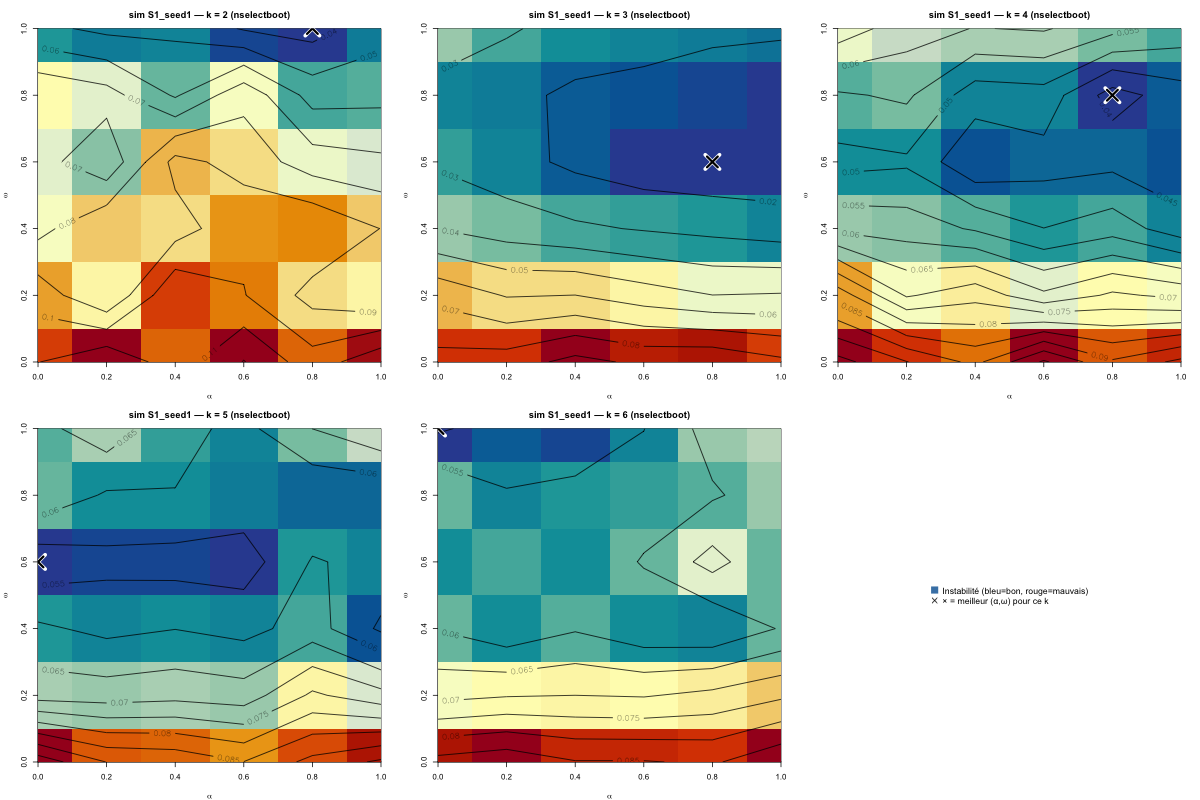
\includegraphics[width=\linewidth]{nselectboot_heatmap_sim_S1_seed1.png}
    \caption{S1 : signal fort sur $(\delta_1,\delta_2,\delta_3)$.}
    \label{fig:instab_sim_S1}
  \end{subfigure}\hfill
  \begin{subfigure}[t]{0.49\textwidth}
    \centering
    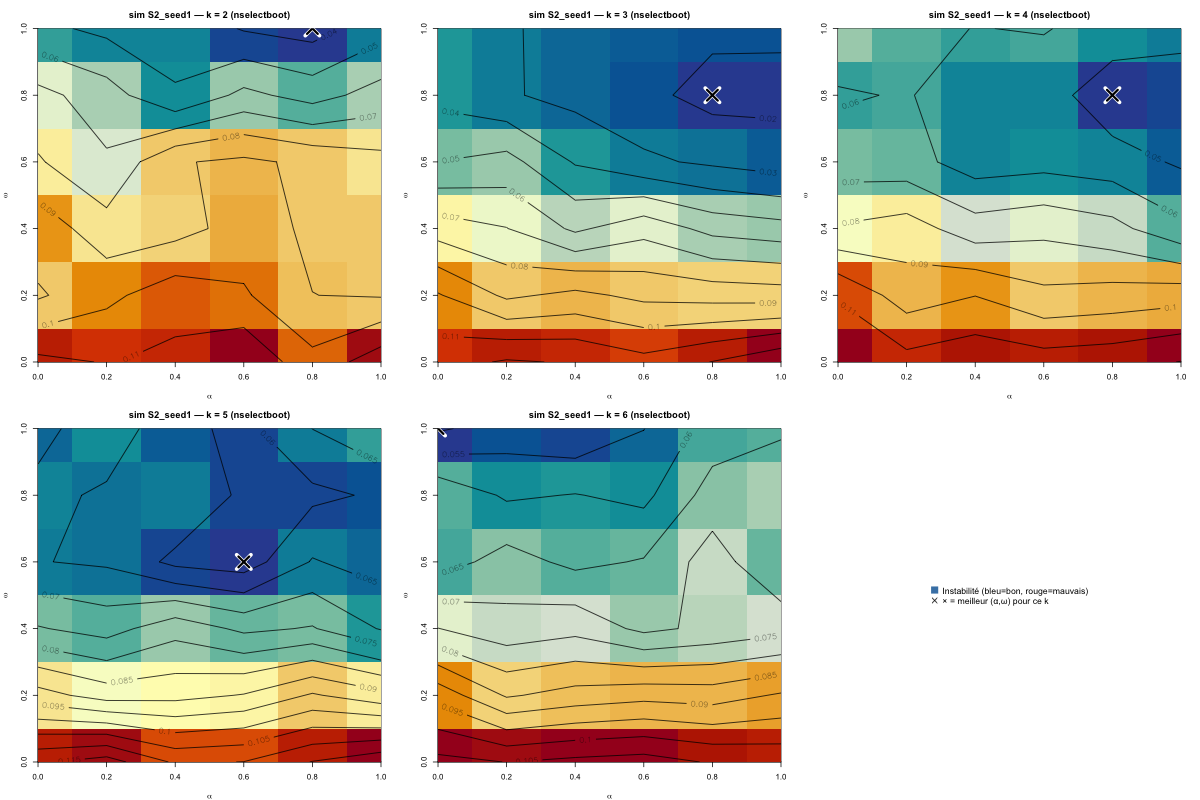
\includegraphics[width=\linewidth]{nselectboot_heatmap_sim_S2_seed1.png}
    \caption{S2 : affaiblissement de $\delta_3$.}
    \label{fig:instab_sim_S2}
  \end{subfigure}

  \vspace{0.6em}

  \begin{subfigure}[t]{0.49\textwidth}
    \centering
    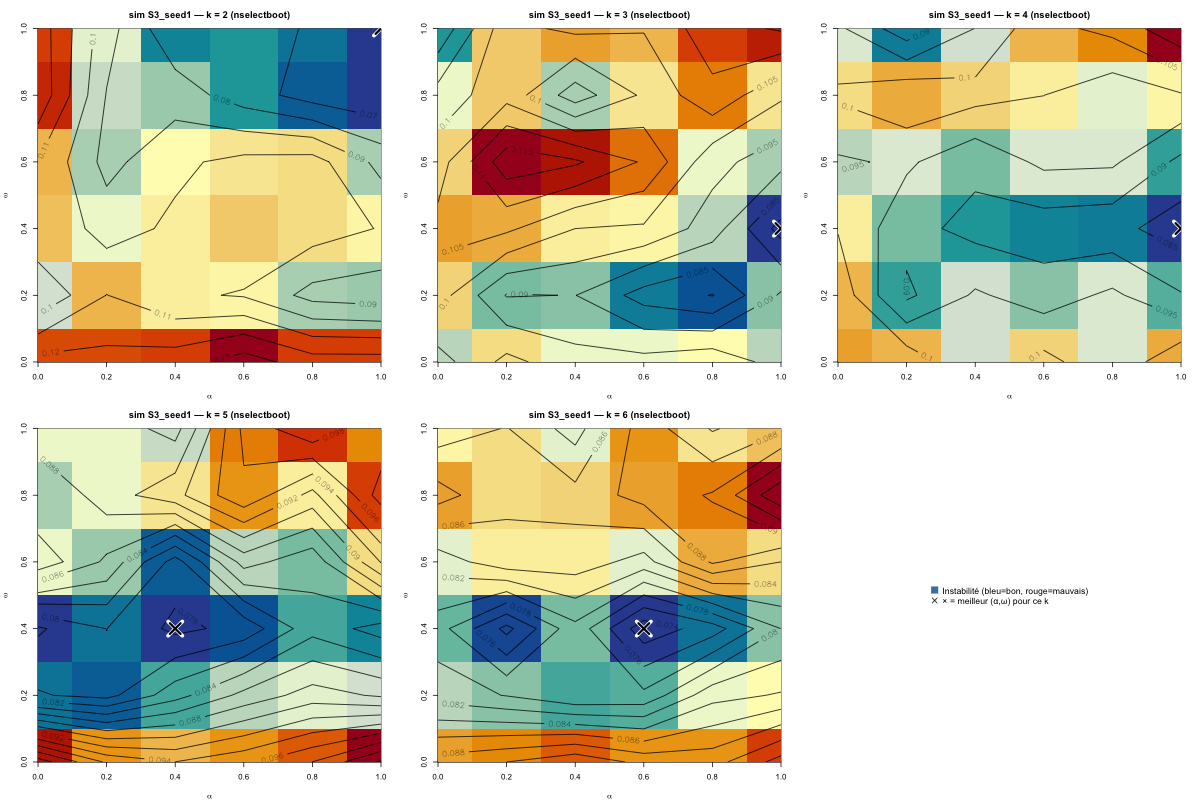
\includegraphics[width=\linewidth]{nselectboot_heatmap_sim_S3_seed1.png}
    \caption{S3 : affaiblissement fonctionnel ($\delta_1,\delta_2$).}
    \label{fig:instab_sim_S3}
  \end{subfigure}\hfill
  \begin{subfigure}[t]{0.49\textwidth}
    \centering
    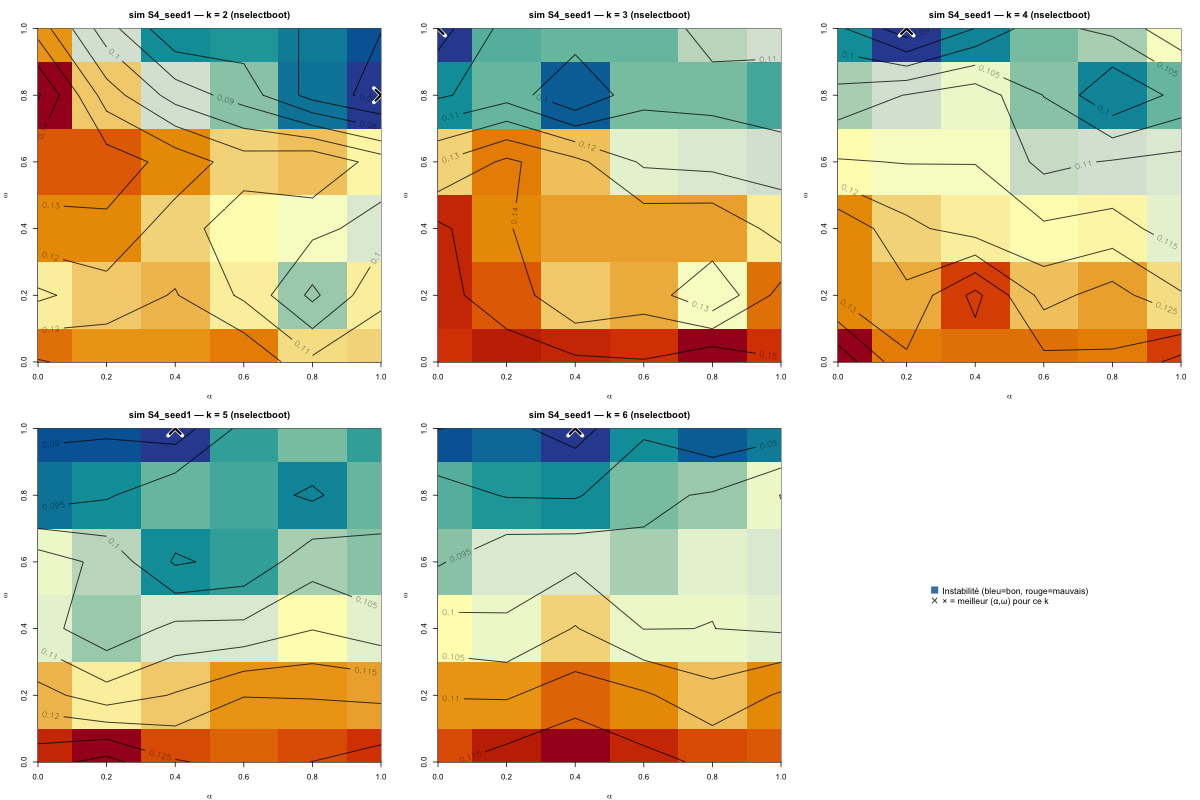
\includegraphics[width=\linewidth]{nselectboot_heatmap_sim_S4_seed1.png}
    \caption{S4 : affaiblissement global.}
    \label{fig:instab_sim_S4}
  \end{subfigure}
  \caption{Données simulées (même protocole $B=150$, grille $21\times 21$, $k\in\{2,\ldots,6\}$)~:
  cette figure montre que l'alignement entre faible instabilité et le vrai $K=3$ se dégrade
  quand les $\delta$ du générateur \texttt{Cas2\_deriv} (section~\ref{sec:materiel}) passent du régime favorable (S1-S2) au régime difficile (S3-S4). Lecture identique à la figure~\ref{fig:instab_reels}.}
  \label{fig:instab_simule}
\end{figure}

\subsection{Scénarios S1 à S4~: interprétation du signal}

Les triplets $\delta$ sont ceux du tableau~\ref{tab:materiel_experimental}.

\paragraph{S1 : $(1,1,1)$.} Signal fort sur les trois leviers~; le classement
ARI met en tête la stratégie~C ($\DK$ surface), puis la chaîne HFV$+\DK$, puis
les approches qui partagent les mêmes scores sur $D_1$ et la stratégie~B
(tableau~\ref{tab:ari_scenarios}).

\paragraph{S2 : $(1,1,0.5)$.} Même intensité fonctionnelle que S1, mais $\delta_3$
réduit la séparation entre moyennes de $Z$~; la stratégie~C reste en tête,
 suivie des blocs $D_1$ / B / $D_f$ à ARI identique, puis $D_0$ et la chaîne
HFV. La stratégie~A se dégrade (signal vectoriel moins marqué).

\paragraph{S3 : $(0.5,0.5,1)$.} Fonctionnel affaibli, vectoriel fort~: le classement
se renverse. La stratégie~A domine, suivie de $D_s$ puis de la stratégie~C~;
les méthodes fortement ancrées sur la forme fonctionnelle chutent.

\paragraph{S4 : $(0.5,0.5,0.5)$.} Affaiblissement global~: le meilleur ARI
moyen est atteint par la baseline $D_1$, suivie de la stratégie~C et de la
stratégie~A~; toutes les valeurs restent basses, ce qui traduit le
caractère frontière du scénario.

\subsection{Comparaison des stratégies~: tableau récapitulatif (ARI moyen)}

Le tableau~\ref{tab:ari_scenarios} synthétise l'ARI moyen de chaque méthode sur
les quatre scénarios. Les
hyperparamètres relevant de la silhouette sont fixés comme dans le pipeline~;
l'ARI n'intervient qu'en \emph{évaluation a posteriori}.

% ---------------------------------------------------------------------------
% Fichier généré — NE PAS ÉDITER À LA MAIN
% Source : experiments/03_simulated_hybride/results/metrics_summary_by_scenario_method.csv
%        + experiments/03_simulated_hybride/results/metrics_global_average_by_method.csv
% Généré le : 2026-03-22 13:23:28 CET
% Git : 394a048
% Regénérer : Rscript scripts/generate_rapport_stage_benchmark_tex.R
% ---------------------------------------------------------------------------

\begin{table}[H]
\centering
\renewcommand{\arraystretch}{1.25}
\begin{tabular}{lcccc|c}
  \toprule
  \textbf{Méthode} & \textbf{S1} & \textbf{S2} & \textbf{S3} & \textbf{S4} & \textbf{Moy. glob.} \\
  \midrule
  Baseline $D_0$ & 0{,}830 & 0{,}830 & 0{,}226 & 0{,}226 & 0{,}528 \\
  Baseline $D_s$ & 0{,}567 & 0{,}333 & 0{,}511 & 0{,}247 & 0{,}414 \\
  Stratégie A (FPCA$+Z$) & 0{,}782 & 0{,}524 & 0{,}623 & 0{,}315 & 0{,}561 \\
  Stratégie B ($\Dw$, sil.) & 0{,}873 & 0{,}873 & 0{,}239 & 0{,}238 & 0{,}556 \\
  Stratégie C ($\DK$ surface) & 0{,}938 & 0{,}887 & 0{,}464 & 0{,}317 & 0{,}651 \\
  Baseline $D_1$ & 0{,}873 & 0{,}873 & 0{,}378 & 0{,}378 & 0{,}626 \\
  $D_f(\alpha)$ (sil.) & 0{,}873 & 0{,}873 & 0{,}237 & 0{,}237 & 0{,}555 \\
  HFV $+$ $\DK$ (reconstr.) & 0{,}897 & 0{,}802 & 0{,}433 & 0{,}301 & 0{,}608 \\
  \bottomrule
\end{tabular}
\caption{ARI moyen par scénario et par méthode ($50$ répétitions par scénario,
  $n=300$, $K=3$, $p=20$). Grille $\alpha$ (et $(\alpha,\omega)$ pour la stratégie~B)
  : $21$ valeurs sur $[0,1]$ (pas $0{,}05$, soit $21\times 21$ couples pour~B).
  Hyperparamètres choisis par silhouette (stratégies B, C, $D_f(\alpha)$)~;
  l'ARI sert uniquement à l'évaluation.
  \emph{Moy. glob.}~: moyenne sur l'ensemble des $200$ runs ($4\times 50$), fichier
  \texttt{metrics\_global\_average\_by\_method.csv}.}
\label{tab:ari_scenarios}
\end{table}



\paragraph{Lecture globale.}
Les moyennes globales confirment l'ordre de grandeur attendu~: stratégie~C
($\approx 0{,}65$), puis $D_1$ et la chaîne HFV$+\DK$ ($\approx 0{,}61$-$0{,}63$),
puis la stratégie~A ($\approx 0{,}56$). Les baselines $D_0$ et $D_s$ sont plus
sensibles au scénario (voir S2-S3). En résumé, sur la moyenne des quatre
scénarios, nous retenons la stratégie~C comme approche de surface la plus
régulièrement compétitive lorsque fonctionnel et vectoriel portent ensemble le
signal (S1-S2)~; nous rappelons toutefois que S3 renverse l'ordre au profit de
A et $D_s$ lorsque seul le vecteur reste informatif.

\subsection{Effondrement en S4~: transparence sur les limites}

Pour S4 ($\delta = (0{,}5, 0{,}5, 0{,}5)$), les ARI du
tableau~\ref{tab:ari_scenarios} chutent simultanément~: la meilleure moyenne
est celle de $D_1$ ($\approx 0{,}38$), suivie de la stratégie~C ($\approx
0{,}32$) et de la stratégie~A ($\approx 0{,}32$). La chaîne HFV$+\DK$ se situe
juste derrière ($\approx 0{,}30$). Ce constat s'interprète clairement~: aucune
des architectures développées dans ce mémoire ne \emph{restaure} une structure absente au niveau du
générateur. Une piste naturelle, non menée ici faute de temps, serait une
pondération adaptative des modalités ou des distances en fonction d'un diagnostic
de rapport signal\,/\,bruit, plutôt qu'un $\omega$ ou un $\alpha$ choisis sur
toute la grille avec les mêmes poids du début à la fin de l'étude.

\subsection{Paradoxe silhouette\,/\,ARI sur les données simulées}
Le tableau~\ref{tab:ari_scenarios} juxtapose, pour chaque scénario et en moyenne
globale, l'ARI (évaluation) et la silhouette moyenne $\bar{s}$ sur les mêmes
runs. On y lit le même type d'écart qu'en données réelles~: le choix par
silhouette sur la stratégie~B (forte $\bar{s}$ sur $D_1$ / $D_f$ en S1-S2) ne
coïncide pas avec le meilleur ARI~; les approches noyau $\DK$ / HFV$+\DK$
affichent des $\bar{s}$ plus modestes tout en restant compétitives au sens de
l'ARI. Maximiser la cohérence géométrique interne ne coïncide donc pas avec la
récupération des classes lorsque celles-ci existent pour l'évaluation.

\medskip
\noindent
En synthèse sur les données simulées~: la stratégie~C et les constructions autour de
$\Dp(\alpha)$ restent les plus utiles lorsque le signal est partagé entre
fonctionnel et vectoriel~; dès que l'une des deux sources faiblit fortement (S3
ou S4), il faut accepter soit un autre classement de méthodes, soit des ARI
bas : ce n'est pas un défaut d'implémentation mais une limite du réglage
fixe adopté.

% ---------------------------------------------------------------------------
\section{Chapitre 6 : Jeux réels étiquetés}
% ---------------------------------------------------------------------------

\subsection{Résultats comparatifs (trois jeux)}

% ---------------------------------------------------------------------------
% Fichier généré — NE PAS ÉDITER À LA MAIN
% Généré le : 2026-03-24 12:05:33 CET
% Git : f2b3ac8
% Source : docs/exports/comparaison_*.csv (CNAM_EXPORT_COMPARAISON=1 + src/main.R)
% Regénérer : CNAM_EXPORT_COMPARAISON=1 pour canadian, growth, tecator puis
%             Rscript scripts/generate_ch6_three_games_table_tex.R
% ---------------------------------------------------------------------------

\begin{table}[H]
  \centering
  \small
  \renewcommand{\arraystretch}{1.25}
  \resizebox{\textwidth}{!}{%
  \begin{tabular}{ll cc cc cc cc cc cc}
    \toprule
    & & \multicolumn{2}{c}{$D_0$} & \multicolumn{2}{c}{$D_s$}
    & \multicolumn{2}{c}{A} & \multicolumn{2}{c}{B ($\Dw$)} & \multicolumn{2}{c}{C ($\DK$)}
    & \multicolumn{2}{c}{HFV$+\DK$} \\
    \cmidrule(lr){3-4}\cmidrule(lr){5-6}\cmidrule(lr){7-8}\cmidrule(lr){9-10}\cmidrule(lr){11-12}\cmidrule(lr){13-14}
    \textbf{Jeu} & $n$ / $k$ & Sil. & ARI & Sil. & ARI & Sil. & ARI & Sil. & ARI & Sil. & ARI & Sil. & ARI \\
    \midrule
  Canadian Weather & 35 / 4 & 0{,}285 & 0{,}229 & 0{,}448 & 0{,}616 & 0{,}395 & 0{,}748 & 0{,}448 & 0{,}616 & 0{,}329 & 0{,}686 & 0{,}332 & 0{,}686 \\
  Growth & 93 / 2 & 0{,}402 & 0{,}115 & 0{,}554 & 0{,}424 & 0{,}360 & 0{,}682 & 0{,}554 & 0{,}424 & 0{,}261 & 0{,}368 & 0{,}273 & 0{,}368 \\
  Tecator & 215 / 3 & 0{,}509 & 0{,}151 & 0{,}476 & 0{,}546 & 0{,}403 & 0{,}439 & 0{,}509 & 0{,}151 & 0{,}265 & 0{,}371 & 0{,}284 & 0{,}374 \\
    \bottomrule
  \end{tabular}
  }
  \caption{Résultats sur trois jeux publics.
  Stratégies B et C~: $(\alpha,\omega)$ ou $\alpha$ choisis par silhouette.
  Colonne \emph{HFV$+\DK$}~: reconstruction par ACP hybride (covariance croisée) puis distance à noyau sur courbes reconstruites et~$Z$ (chapitre~3).}
  \label{tab:resultats_reels}
\end{table}



\subsection{Interprétation}

\paragraph{Stratégie A (FPCA$+Z$, k-means) et ligne de base.}
Sur Canadian Weather et Growth, la stratégie~A atteint le meilleur ARI du
tableau~\ref{tab:resultats_reels}. Sur Tecator, c'est la baseline $D_s$
(seul bloc vectoriel) qui maximise l'ARI ($0{,}546$)~: le signal discriminant
y est surtout porté par les covariables chimiques, ce qui relativise
l'apport de la forme spectrale pour cette étiquette de classe. La chaîne
HFV$+$ $\DK$ se situe au même ordre de grandeur que la stratégie~C sur les
trois jeux et rejoint l'ARI de~C sur Canadian Weather ($0{,}686$), ce qui
illustre le rôle de la covariance croisée lorsque les deux modalités sont
jointement informatives.

\paragraph{Paradoxe silhouette / ARI sur données réelles.}
Pour la stratégie~B, le couple $(\alpha,\omega)$ maximisant la silhouette
diverge systématiquement du couple qui maximiserait l'ARI~: la silhouette
sélectionne des configurations proches des baselines pures ($\omega \in \{0,1\}$)
plutôt que des mélanges hybrides équilibrés. Ce constat reproduit le paradoxe
documenté en section~\ref{sec:silhouette} et s'observe de façon cohérente sur les trois jeux.

\paragraph{Poids de la forme ($D_1$) sous optimisation ARI.}
Sur les trois jeux, le paramètre $\alpha$ maximisant l'ARI (évaluation \emph{a
posteriori} par ARI uniquement) satisfait $\alpha \geq 0{,}6$~: la dynamique de forme est
systématiquement plus discriminante que le seul niveau vertical. Cette
observation confirme le rôle informatif de $D_1$ pour les stratégies qui
utilisent explicitement $\mathcal{D}_p(\alpha)$ et plaide pour ne pas fixer
$\alpha = 0$ par défaut en mode opérationnel.

% ---------------------------------------------------------------------------
\section{Conclusion générale}
% ---------------------------------------------------------------------------

Le problème abordé dans ce mémoire a été d'explorer le couplage entre données fonctionnelles et vectorielles pour le clustering non supervisé. L'étude empirique a démontré que l'ACP hybride (HFV) construite conjointement avec les distances noyaux constitue une alternative robuste et très interprétable face aux stratégies classiques d'hybridation (méthodes A, B, C). Toutefois, aucune stratégie ne domine universellement : la performance reste logiquement subordonnée à la localisation du signal discriminant (forme de la courbe ou covariables de l'espace vectoriel).

Au-delà de ces comparaisons, la véritable complexité soulevée reste d'ordre structurel. L'expérience a mis en évidence le paradoxe entre la silhouette (mesure géométrique interne) et l'ARI (vérité terrain) : la recherche aveugle du meilleur compromis mathématique sans labels tend à écraser l'une des dimensions et à créer des clusters artificiels. C'est ici que se trouve le cœur scientifique et les perspectives de ce sujet : comment concevoir des algorithmes non-supervisés ou des heuristiques capables d'explorer intelligemment un ratio de variances inter-modalités \emph{sans} la myopie des critères internes traditionnels ?

% ---------------------------------------------------------------------------
% Bibliographie
% ---------------------------------------------------------------------------
\begin{thebibliography}{9}

\bibitem{ferreira}
Ferreira, L., \& de Carvalho, F. A. (2014). \textit{A novel approach to clustering mixed data}.

\bibitem{fang}
Fang, Y., \& Wang, J. (2012). \textit{Selection of the number of clusters via the bootstrap method}.

\end{thebibliography}

\end{document}
